\documentclass[xcolor=dvipsnames, 10pt]{beamer}
\usepackage[utf8]{inputenc}
\usepackage{enumitem,xcolor}
% \usetheme{CambridgeUS}
\usepackage{libertine}
\usepackage{enumerate}
\usepackage{booktabs}

\usepackage{MnSymbol,wasysym}
\usepackage{ragged2e}
\usepackage{threeparttable}
\justifying

\definecolor{blue}{HTML}{1a296b}
% \definecolor{lightblue}{HTML}{009bbd}
\definecolor{lightblue}{RGB}{86,76,169}
\definecolor{grey}{HTML}{C3C5C2}
\definecolor{white}{HTML}{FDFEFE}
\definecolor{darkred}{rgb}{0.8,0,0}
\definecolor{myGrey}{rgb}{.7,.7,.7}
\usepackage{color}
\definecolor{twi}{RGB}{86,76,169}
\definecolor{TWI}{RGB}{86,76,169}
\newcommand{\old}[1]{{\color{myGrey} #1\color{black}}}
\newcommand{\orange}[1]{{\color{orange} #1\color{black}}}
\newcommand{\iw}[1]{{\color{blue} #1\color{black}}}
\newcommand{\twi}[1]{{\color{TWI} #1\color{black}}}


\setbeamercolor{normal text}{fg=black,bg=white}
\setbeamercolor{alerted text}{fg=blue}
\setbeamercolor{example text}{fg=black}
\setbeamercolor{title}{fg=TWI}
\setbeamercolor{frametitle}{fg=TWI}
\setbeamercolor{structure}{fg=TWI}
% \setbeamercovered{dynamic}
% \setbeamercovered{transparent=5}
\setbeamercovered{%
still covered={\opaqueness<1>{4}\opaqueness<2>{2}\opaqueness<3>{1}\opaqueness<4->{1}},
again covered={\opaqueness<1->{50}}}
\setbeamertemplate{navigation symbols}{}

\setbeamercolor{palette primary}{fg=white, bg=blue}
\setbeamercolor{palette secondary}{fg=white, bg=blue}
\setbeamercolor{palette tertiary}{fg=white, bg=lightblue}

\setbeamercolor{button}{bg=blue,fg=white}

\setlist[itemize,1]{label=$\color{lightblue}\blacktriangleright$}
\setlist[itemize,2]{label=\boldmath$\color{lightblue}\cdot$}

\usepackage{caption}
% \usepackage[labelfont={color=blue}]{caption}
% \makeatletter
% \setbeamertemplate{title page}[default][colsep=-4bp,rounded=true]
% \setbeamertemplate{footline}{%
%     \leavevmode%
%     \hbox{%
%         \begin{beamercolorbox}[wd=.2\paperwidth,ht=2.25ex,dp=1ex,center]{author in head/foot}%
%             \usebeamerfont{author in head/foot}\insertshortauthor\expandafter\beamer@ifempty\expandafter{\beamer@shortinstitute}{}{~~(\insertshortinstitute)}
%         \end{beamercolorbox}%
%         \begin{beamercolorbox}[wd=.6\paperwidth,ht=2.25ex,dp=1ex,center]{title in head/foot}%
%             \usebeamerfont{title in head/foot}\insertshorttitle
%         \end{beamercolorbox}%
%         \begin{beamercolorbox}[wd=.2\paperwidth,ht=2.25ex,dp=1ex,right]{date in head/foot}%
%             \usebeamerfont{date in head/foot}\insertshortdate{}\hspace*{2em}
%             \insertframenumber{} / \inserttotalframenumber\hspace*{2ex}
%         \end{beamercolorbox}}%
%         \vskip0pt%
%     }
% \makeatother

\setbeamertemplate{headline}{}
\setbeamertemplate{footline}{}

\title[Title]{\textbf{When personalization deters delegation to
		algorithms:\\ Evidence from a preregistered
		experiment}}
\author[I.Wolff\hspace{1.3cm}]{Irenaeus Wolff\\\vspace{.2cm}\footnotesize Thurgau Institute of Economics (TWI), \\University of Konstanz}
\date[Wolff @ AI WS 2026]{AI Workshop (Berlin), 23$^{\text{rd}}$ June, 2026}

% \logo{\includegraphics[scale = .17]{TWI_logo_for_presentations_TITLE_bg.pdf}\vspace{220pt} \hspace{-.15cm}}


\begin{document}
\logo{
\includegraphics[scale = .37]{logo_twi_cmyk.pdf}\vspace{220pt} \hspace{-.15cm}}
% THIS IS THE TITLEFRAME
\frame{
	\vspace{4.0cm}
	{\LARGE \twi{When personalization deters delegation to algorithms: Experimental evidence}}%\vspace{.2cm}}\\ 
\\
\vspace{.5cm}
{\large Lara Suraci \& Irenaeus Wolff}\vspace{.1cm}\\
{\small  --- 23$^\text{rd}$ June, 2026, Symposium on `AI and the Future of Work', Berlin ---}
}

\logo{}


%This redefines the background for the regular slides(i.e. the smaller logo in the top-right corner)
\logo{
\includegraphics[scale = 0.25]{logo_twi_cmyk.pdf}\vspace{225pt} \hspace{-.12cm}}


%
% \author[Lara Suraci]{Lara Suraci \newline with Robin Cubitt, Chris Starmer and Irenaeus Wolff}
% \date[]{19 April 2023}
%
% \AtBeginSection[]
% {
%   \begin{frame}
%     \frametitle{Table of Contents}
%     \tableofcontents[currentsection]
%   \end{frame}
% }
%
% \begin{document}
% \setbeamertemplate{section in toc}[sections numbered]
%
% 	\begin{frame}
% 	\titlepage
% \centering
% \includegraphics[scale=0.33]{notts_logo2.png}
% 	\end{frame}


\frame{\frametitle{Background}
 \begin{itemize}
  \item Huge \& unconnected literature on algorithm/automation/AI/... reliance ($\rightarrow$ review by Chugunova \& Sele, 2022)
  \item Most of the literature: setups with clearly identifiable mistakes
  \item But in many real-life settings, preferences determine what is a mistake
  \item E.g., robo-advisors: maximal payoff \textit{vs} best fit to risk-parameters
%   \item[\twi{$\rightarrow$}]<2-> Our (first) research question!
%   \item[\twi{No. 2:}]<2-> What are the consequences of feedback under either variant?
%   \item[\twi{$\rightarrow$}]<2->  overweighting of algorithmic errors (Madhavan \& Wiegmann, 2007; Dietvorst et al. 2015; Hoff \& Bashir, 2015)
 \end{itemize}
}

\frame{\frametitle{Relevance?}
 Well-known (Swiss) robo-advisors(' marketing strategies)
 \begin{itemize}
  \item ``We rely on a low-cost, passive investment strategy and have selected a total of 9 equity, bond and real estate ETFs from over 1,500 ETFs (exchange-traded funds) and put them together in such a way that they \twi{achieve an optimal risk/return ratio}.'' (findependent.ch; for GER, see e.g., whitebox.eu)
  \item ``Chat with Selma: Selma \twi{looks at your financial life and learns how you should structure your finances}. Get your plan: Selma \twi{creates a personalized investment plan that fits your life}. Sit back and relax! Selma takes care of your money from now on and does all the buying and selling for you.'' (selma.com; for GER, see e.g., quirion.de)
 \end{itemize}
}

  \frame{\frametitle{Research Question}
    \begin{itemize}
	     \item Does algorithm reliance differ for \textcolor{lightblue}{\textbf{objective optimization  \textit{vs.} preference-based personalisation}} in a preferential-choice environment?%\vspace{.2cm}
	     \begin{itemize}
	     	\item[(i)] ...at first contact?
	     	\item[(ii)] ...overall?
	     \end{itemize}
    \end{itemize}
  }

   \begin{frame}
	\frametitle{Objective vs Personalised Algorithms}%\vspace{1.5cm}}
	\begin{itemize}
	\setlength\itemsep{1em}
 %\item in BB, I will call it normative but just explain that this can be discussed “only a label, not an assertion that it is rational to be risk-averse” (same for PT, attempt to capture parameters, no one is asserting that PT is perfect as a model)
  \item What do we mean by \textcolor{lightblue}{\textbf{objective optimization}}?%\\\smallskip
  \begin{itemize}
   \item an algorithm that chooses some ‘objectively ideal’ option independently of a subject’s preferences (here: \textcolor{lightblue}{\textbf{highest EV}})\vspace{-.2cm}
  \end{itemize}
  \item What do we mean by \textcolor{lightblue}{\textbf{personalised}}?%\\\smallskip
  \begin{itemize}
   \item an algorithm that measures a subject’s preferences and chooses accordingly (here: \textcolor{lightblue}{\textbf{implementation of revealed preferences}})\vspace{-.2cm}
  \end{itemize}
 \end{itemize}
\end{frame}


     \begin{frame}
	\frametitle{Objective vs Personalised Algorithms\vspace{.3cm}}
	\begin{itemize}
	\setlength\itemsep{1em}
 %\item in BB, I will call it normative but just explain that this can be discussed “only a label, not an assertion that it is rational to be risk-averse” (same for PT, attempt to capture parameters, no one is asserting that PT is perfect as a model)
	\item What do we mean by \textcolor{lightblue}{\textbf{objective optimization}}?%\\\smallskip
  \begin{itemize}
	\item an algorithm that chooses some ‘objectively ideal’ option independently of a subject’s preferences (here: \textcolor{lightblue}{\textbf{highest EV}})\vspace{-.2cm}
   \end{itemize}
	\item What do we mean by \textcolor{lightblue}{\textbf{personalised}}?%\\\smallskip
  \begin{itemize}
	\item an algorithm that measures a subject’s preferences and chooses accordingly (here: \textcolor{lightblue}{\textbf{implementation of revealed preferences}})\vspace{-.2cm}
  \end{itemize}
	\item In the experiment, we describe both algorithms in intuitive terms:\\\medskip \textcolor{lightblue}{\textbf{EV}}: \textit{‘The algorithm works out how much each option would yield on average and selects the option for which this is highest.’}\\\smallskip
  \textcolor{lightblue}{\textbf{Prefs}}: \textit{‘The algorithm analyses your choices from Part 1 and selects the best option for you in light of your Part-1 choices.’}
 	\end{itemize}
 	\end{frame}


 		\begin{frame}
	\frametitle{Experimental Design}%\vspace{2.5cm}}
	\begin{itemize}
	\setlength\itemsep{1em}
 	\item[\textcolor{lightblue}{\textbf{Part 1}}] \textcolor{lightblue}{-- } Elicitation of preferences
 	 \begin{itemize}
 	 	 \item ordered lotteries, no foils, unlimited time
 	 	 \item ``hypothetical, but the choices may be meaningful for Part 2''
 	 \end{itemize}
   \item[\textcolor{lightblue}{\textbf{Part 2}}] \textcolor{lightblue}{-- } Lottery Selection Task
    \begin{itemize}
     \item could stand for an investment task
     \item complexity (number of options, outcomes under different SOTW)
     \item time pressure (think: relative to the number of options)
%      \item robo-advisors: opaque, `personalisable', supposedly `optimal'
    \end{itemize}

 	\end{itemize}
 	\end{frame}

	\frame{\frametitle{Tasks}
		\begin{figure}
			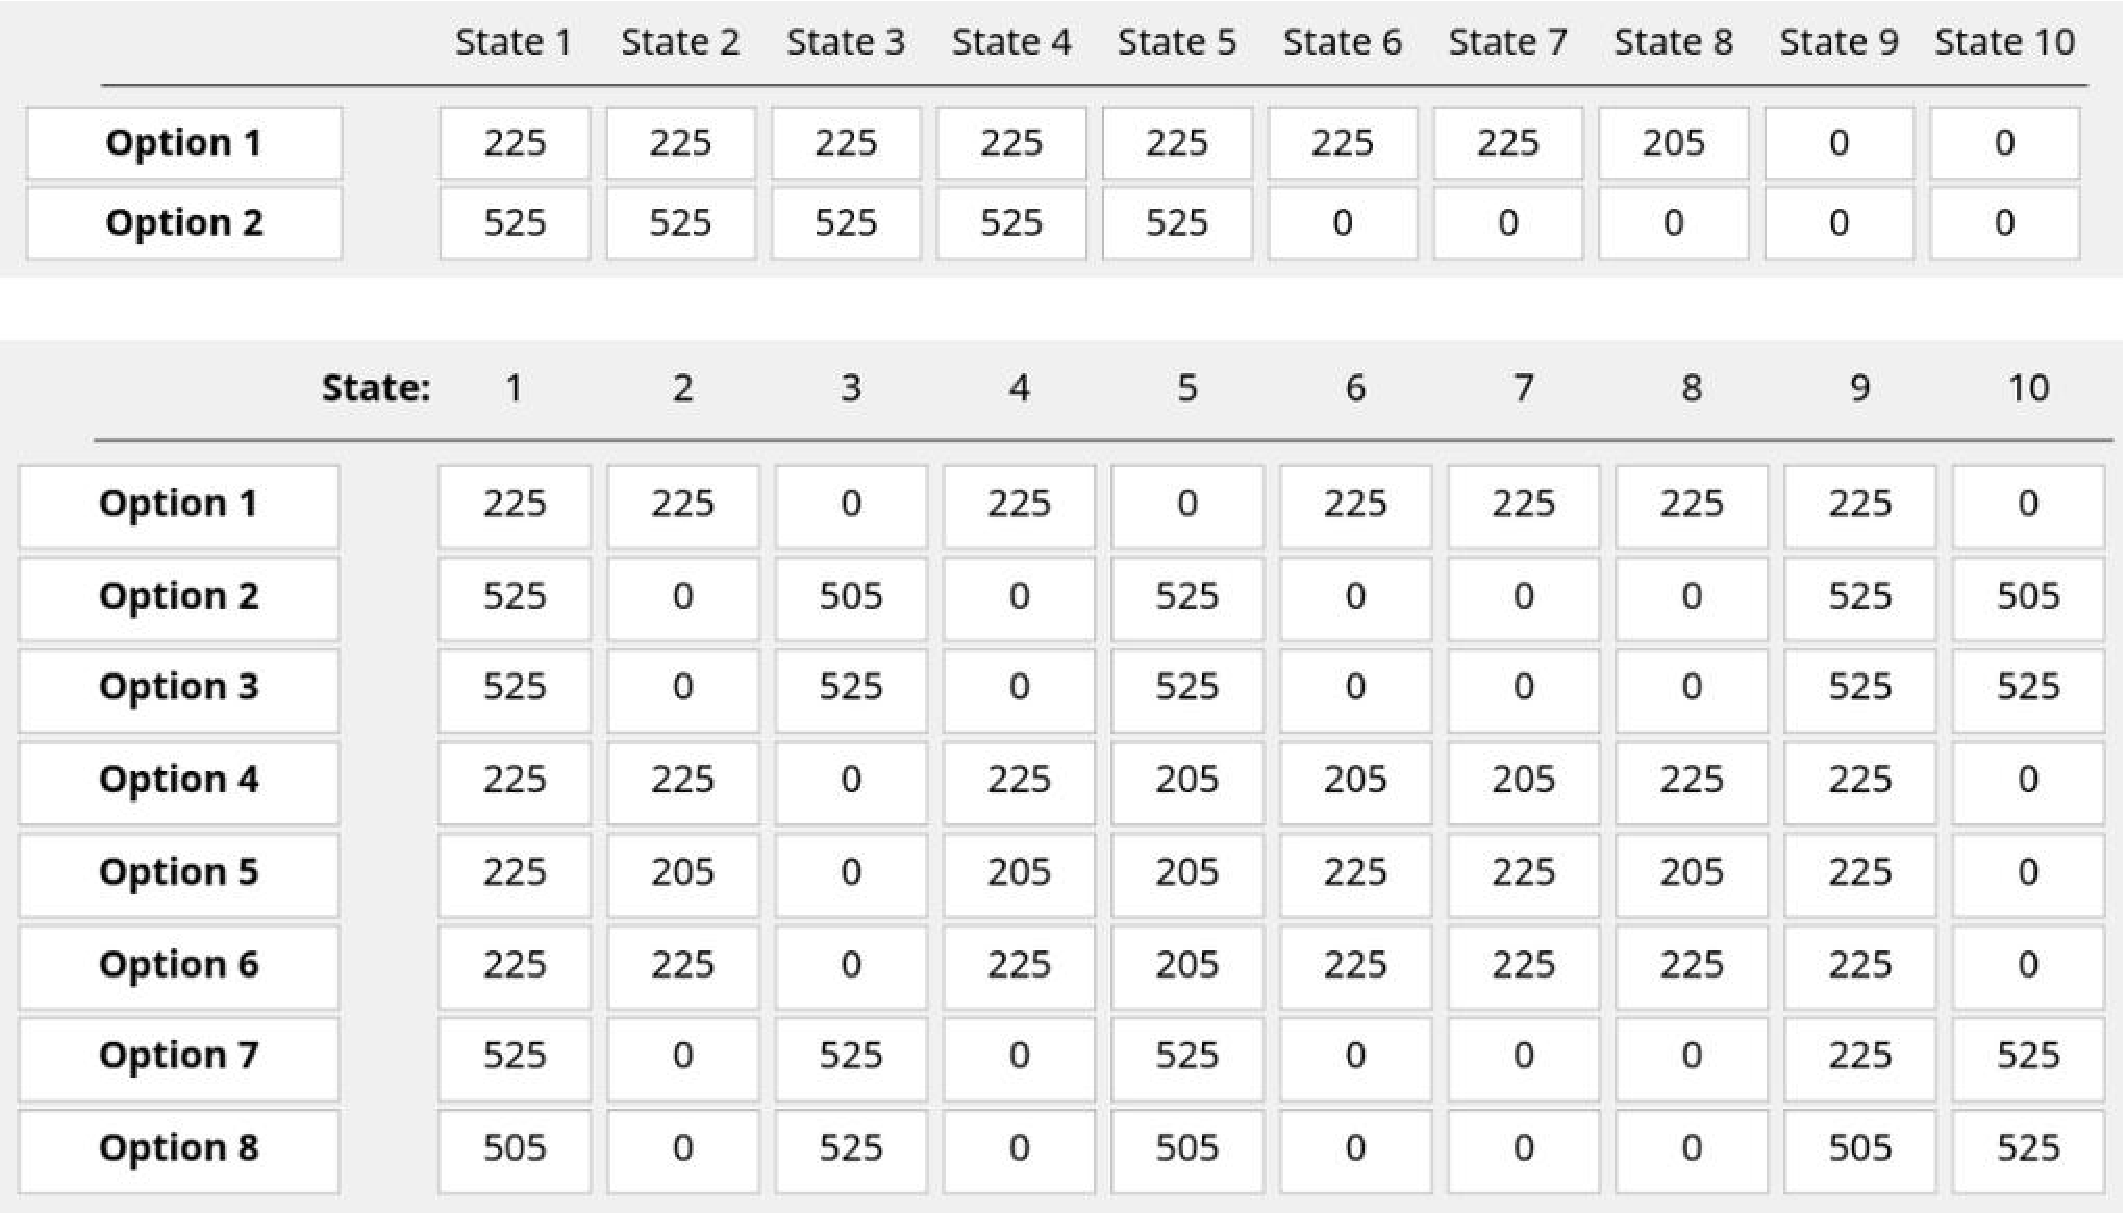
\includegraphics[width = .8\textwidth]{Figure_ExampleScreens.pdf}
		\end{figure}
		\begin{itemize}
			\item<2-> For further distraction: 4 filler tasks in between
			\item 8 rounds: 5' pre-view --- 5' algorithm choice---8' decision/waiting time\vspace{-.2cm}
		\end{itemize}
	}

	\frame{\frametitle{Main Results: First Contact}
		\begin{itemize}
			\item \textbf{Hypothesis:} Higher delegation to EV-maximizing algorithm than to personalized algorithm.
			\item \textbf{Finding:} Supported at first contact.
			\item Delegation rates in Round 1: \textcolor{lightblue}{\textbf{66.9\% (EV)}} vs. \textcolor{lightblue}{\textbf{55.8\% (Prefs)}}.
			\item Boschloo exact test: $p = 0.0413$.
			\item Treatment gap is concentrated in the first decision.
		\end{itemize}
	}

	\frame{\frametitle{Main Results: Repeated Decisions}
		\begin{itemize}
			\item \textbf{Average Delegation:} No significant treatment difference overall ($p = 0.2425$).
			\item \textbf{Dynamics:} Convergence over rounds.
			\item Delegation in EV condition declines more strongly after Round 1.
			\item \textbf{Key Driver:} Negative feedback (specifically prior zero-outcomes) strongly deters subsequent delegation ($\beta = -0.3854, p < 0.001$).
		\end{itemize}
	}

	\frame{\frametitle{Categorical Non-Delegation}
		\begin{itemize}
			\item A distinct acceptance barrier under personalization.
			\item \textbf{Never-delegators:}
			\begin{itemize}
				\item \textcolor{lightblue}{\textbf{15.7\%}} in Preference-based condition.
				\item \textcolor{lightblue}{\textbf{3.4\%}} in EV condition.
			\end{itemize}
			\item Not linked to demographics, risk preferences, or AI experience.
			\item Not linked to dissatisfaction with Part 1 preferences.
		\end{itemize}
	}

	\frame{\frametitle{Mechanisms \& Interpretations}
		\begin{itemize}
			\item \textbf{The "Agency" Trade-off:} Personalization may encroach on users' sense of choice authority.
			\item \textbf{Deterrence Channels:}
			\begin{itemize}
				\item \textit{Personalized:} Deterred by expectation of non-preferred choices.
				\item \textit{EV:} Deterred by expectation of "completely weird" (extreme) choices.
			\end{itemize}
			\item \textbf{Conclusion:} Preference-matching can raise initial hesitation and heighten concerns about autonomy, functioning as an acceptance barrier.
		\end{itemize}
	}

	\frame{\frametitle{Implications for Design}
		\begin{itemize}
			\item Personalization is not a uniformly beneficial acceptance lever.
			\item In high-stakes domains (Finance, Healthcare), objective optimization may face lower initial resistance.
			\item \textbf{Takeaway:} Uptake depends on perceived rule characteristics, not just expected performance.
		\end{itemize}
	}


 	
\end{document}


